%%
% Please see https://bitbucket.org/rivanvx/beamer/wiki/Home for obtaining beamer.
%%
\documentclass[hyperref={pdfpagelabels=false}]{beamer}
\usepackage{lmodern}
%\usetheme{CambridgeUS}
\usetheme{netvor}
\usepackage{color}
\usepackage{gitdags}

\title{git basics}  
\author{Michal \v{S}tembera} 
\titlegraphic{
\includegraphics[height=0.10\textheight]{logo_netvor}}

\date{\today} 
\begin{document}
\begin{frame}
	\titlepage
\end{frame} 


\begin{frame}
\frametitle{Table of contents}
\tableofcontents
\end{frame} 

%
\section{What is git} 
\subsection{Subsection no.1.1}
\begin{frame}
\frametitle{Version Control System (VCS)}
\begin{columns}
\begin{column}{0.4\textwidth}
	\begin{itemize}
		\item Distributed version control
		\item Each client has its copy of history
		\item Database can be altered offline
	\end{itemize}
\end{column}
\begin{column}{0.6\textwidth}  %%<--- here
    \begin{center}
     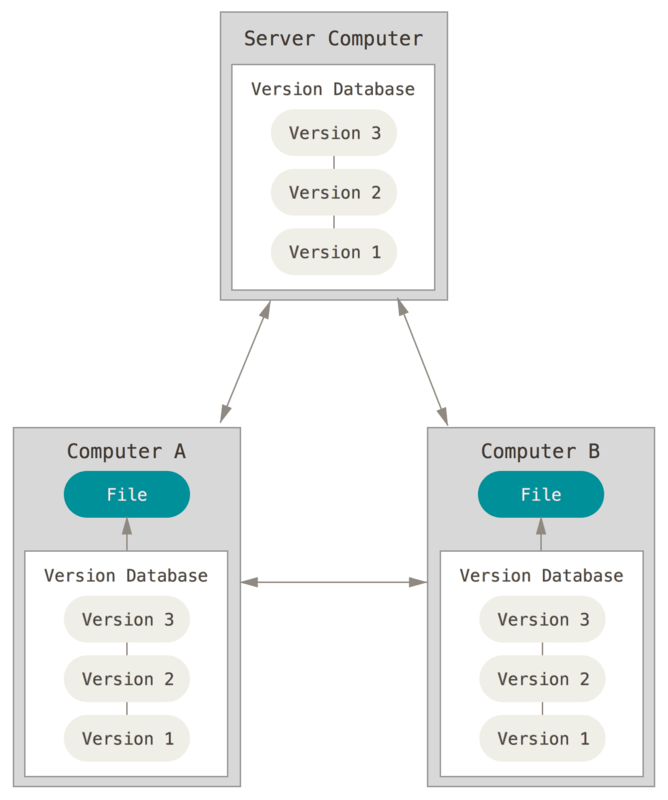
\includegraphics[width=0.6\textwidth]{distributed}
     \end{center}
\end{column} 
\end{columns}
\end{frame}

\begin{frame}
\frametitle{Deltas or snapshot}
\begin{columns}
\begin{column}{0.3\textwidth}
	\begin{itemize}
		\item Exposed as deltas
		\vspace{0.1\textheight}
		\item Internally stored as snapshots
	\end{itemize}
\end{column}
\begin{column}{0.7\textwidth}  %%<--- here
	\begin{center}
    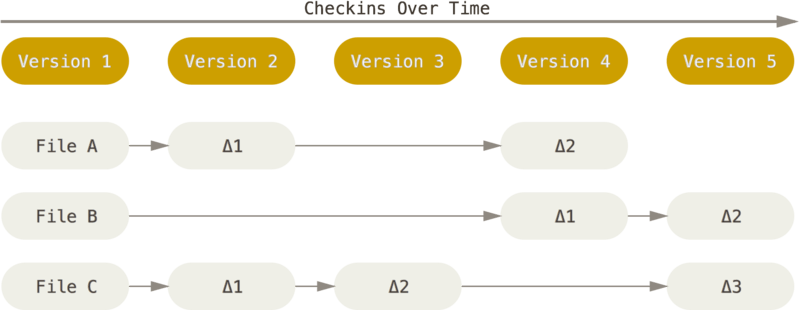
\includegraphics[width=0.8\textwidth]{deltas}
    \vspace{2em}
    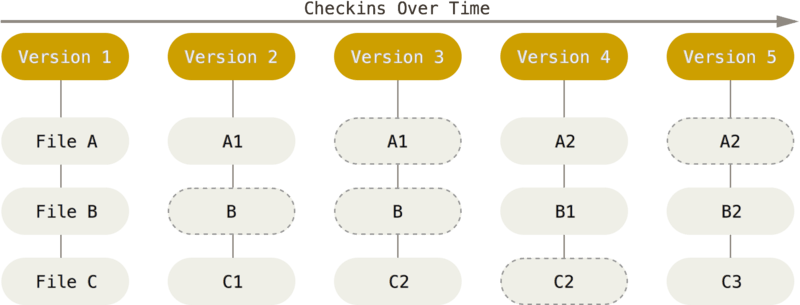
\includegraphics[width=0.8\textwidth]{snapshots}
    \end{center}
\end{column}
\end{columns}
\end{frame}

\begin{frame}
\frametitle{The Three States}
\begin{columns}
\begin{column}{0.4\textwidth}
	\begin{itemize}
		\item Exposed as deltas
		\item Internally stored as snapshots
	\end{itemize}
\end{column}
\begin{column}{0.6\textwidth}  %%<--- here
    \begin{center}
    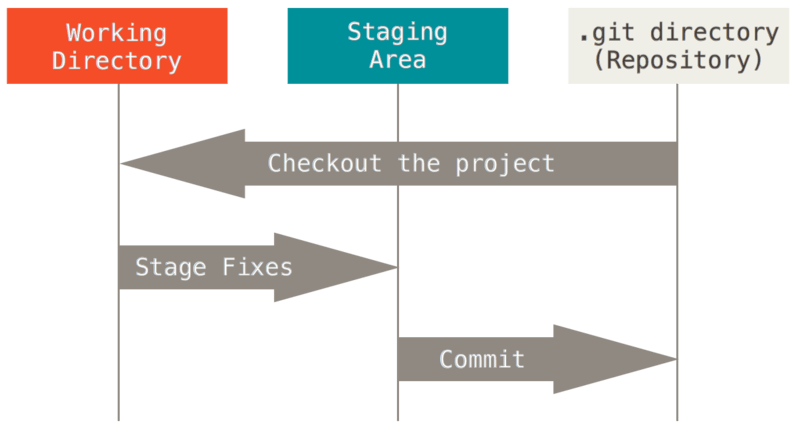
\includegraphics[width=0.6\textwidth]{areas}
    
    \end{center}
\end{column}
\end{columns}
\end{frame}

\begin{frame}
\section{Section no. 2} 
\subsection{Lists I}
\begin{columns}[T]
\column{.5\textwidth}
 \visible<1->{\begin{figure}
    \centering
    \begin{tikzpicture}
      % Commit DAG
      \gitDAG[grow right sep = 2em]{
        A -- B -- { 
          C,
          D -- E,
        }
      };
      % Tag reference
      \gittag
        [v0p1]       % node name
        {v0.1}       % node text
        {above=of A} % node placement
        {A}          % target
      % Remote branch
      \gitremotebranch
        [origmaster]    % node name
        {origin/master} % node text
        {above=of C}    % node placement
        {C}             % target
      % Branch
      \gitbranch
        {master}     % node name and text 
        {above=of E} % node placement
        {E}          % target
      % HEAD reference
      \gitHEAD
        {above=of master} % node placement
        {master}          % target
    \end{tikzpicture}
\end{figure}}
\visible<2->{\begin{figure}
    \centering
    \begin{tikzpicture}
      % Commit DAG
      \gitDAG[grow right sep = 2em]{
        A -- B -- { 
          C,
          D -- E,
        }
      };
      % Tag reference
      \gittag
        [v0p1]       % node name
        {v0.1}       % node text
        {above=of A} % node placement
        {A}          % target
      % Remote branch
      \gitremotebranch
        [origmaster]    % node name
        {origin/master} % node text
        {above=of C}    % node placement
        {C}             % target
      % Branch
      \gitbranch
        {master}     % node name and text 
        {above=of E} % node placement
        {E}          % target
      % HEAD reference
      \gitHEAD
        {above=of master} % node placement
        {master}          % target
    \end{tikzpicture}
\end{figure}}
\column{.5\textwidth}
\visible<3->{\begin{figure}
    \centering
    \begin{tikzpicture}
      % Commit DAG
      \gitDAG[grow right sep = 2em]{
        A -- B -- { 
          C,
          D -- E,
        }
      };
      % Tag reference
      \gittag
        [v0p1]       % node name
        {v0.1}       % node text
        {above=of A} % node placement
        {A}          % target
      % Remote branch
      \gitremotebranch
        [origmaster]    % node name
        {origin/master} % node text
        {above=of C}    % node placement
        {C}             % target
      % Branch
      \gitbranch
        {master}     % node name and text 
        {above=of E} % node placement
        {E}          % target
      % HEAD reference
      \gitHEAD
        {above=of master} % node placement
        {master}          % target
    \end{tikzpicture}
\end{figure}}
\end{columns}
\end{frame}

\begin{frame}\frametitle{lists with single pauses}
\begin{itemize}
\item Introduction to  \LaTeX{}  \pause 
\item Course 2 \pause 
\item Termpapers and presentations with \LaTeX{}  \pause 
\item Beamer class
\end{itemize} 
\end{frame}

\begin{frame}\frametitle{lists with pause}
\begin{itemize}[<+->]
\item Introduction to  \LaTeX{}  
\item Course 2
\item Termpapers and presentations with \LaTeX{}  
\item Beamer class
\end{itemize} 
\end{frame}

\subsection{Lists II}
\begin{frame}\frametitle{numbered lists}
\begin{enumerate}
\item Introduction to  \LaTeX{}   
\item Course 2 
\item Termpapers and presentations with \LaTeX{}  
\item Beamer class
\end{enumerate}
\end{frame}

\begin{frame}
\frametitle{numbered lists with single pauses}
\begin{enumerate}
\item Introduction to  \LaTeX{}  \pause 
\item Course 2 \pause 
\item Termpapers and presentations with \LaTeX{}  \pause 
\item Beamer class
\end{enumerate}
\end{frame}

\begin{frame}
\frametitle{numbered lists with pause}
\begin{enumerate}[<+->]
\item Introduction to  \LaTeX{}  
\item Course 2
\item Termpapers and presentations with \LaTeX{}  
\item Beamer class
\end{enumerate}
\end{frame}




\section{Section no.3} 
\subsection{Tables}
\begin{frame}
\frametitle{Tables}
\begin{tabular}{|c|c|c|}
\hline
\textbf{Date} & \textbf{Instructor} & \textbf{Title} \\
\hline
WS 04/05 & Sascha Frank & First steps with  \LaTeX  \\
\hline
SS 05 & Sascha Frank & \LaTeX \ Course serial \\
\hline
\end{tabular}
\end{frame}


\begin{frame}
\frametitle{Tables with pause}
\begin{tabular}{c c c}
A & B & C \\ 
\pause 
1 & 2 & 3 \\  
\pause 
A & B & C \\ 
\end{tabular} 
\end{frame}


\section{Section no. 4}
\subsection{blocs}
\begin{frame}
\frametitle{blocs}

\begin{block}{title of the bloc}
bloc text
\end{block}

\begin{exampleblock}{title of the bloc}
bloc text
\end{exampleblock}


\begin{alertblock}{title of the bloc}
bloc text
\end{alertblock}
\end{frame}

\end{document}
